\documentclass[11pt,a4paper]{amsart}
\usepackage[utf8]{inputenc}
\usepackage[T1]{fontenc}
\usepackage{lmodern}
\usepackage{amsmath,amssymb,amsthm}
\usepackage{booktabs}
\usepackage{graphicx}
\usepackage[margin=2.3cm]{geometry}
\usepackage{xcolor}
\usepackage[colorlinks=true,linkcolor=blue!50!black,citecolor=blue!50!black,urlcolor=blue!50!black]{hyperref}

\newtheorem{theorem}{Theorem}
\newtheorem{lemma}[theorem]{Lemma}
\newtheorem{proposition}[theorem]{Proposition}
\theoremstyle{remark}
\newtheorem{remark}[theorem]{Remark}
\newtheorem*{remark*}{Remark}

\newcommand{\eps}{\varepsilon}
\renewcommand{\thetable}{A}
\newcommand{\BJS}{\cite{BJS}}

\title[An explicit version of Chen's theorem]{A note on an explicit version of Chen's theorem}
\author{Ruqing Chen}
\address{GUT Geoservice Inc., Montreal, Canada}
\email{ruqing@hotmail.com}
\thanks{Code and data:
\href{https://github.com/Ruqing1963/bordignon-johnston-chen-audit}{github.com/Ruqing1963/bordignon-johnston-chen-audit};
\href{https://doi.org/10.5281/zenodo.24323781}{doi:10.5281/zenodo.24323781}.}
\date{\today}
\subjclass[2020]{11P32, 11N36}
\keywords{Chen's theorem, linear sieve, explicit estimates, Siegel zeros}

\begin{document}
\begin{abstract}
We re-examine the final numerical step of Bordignon, Johnston and Starichkova, \emph{An explicit
version of Chen's theorem and the linear sieve}, Int.\ J.\ Number Theory 21 (2025), and find three issues.
(i)~In the bound for $S(B,P(y))$ the factor $U_N^{-1}$ is replaced by $(2e^{\gamma}C_2)^{-1}=0.4252$, whereas the
definition of $U_N$ only gives $U_N^{-1}\le(2e^{-\gamma}C_2)^{-1}=1.3490$, a factor $e^{2\gamma}$ larger.
(ii)~In the same bound the constant $\eps_2$ is evaluated at $X_3^8$, although the hypothesis it needs is only
available at $X_3$. (iii)~The explicit linear-sieve constants obtained from Lemmas~8--14 are about $25\%$ larger
than those printed in Table~1, and Lemma~14 gives no bound at all for $1/\eps\ge221$. The effect on the lower
bound in the case of a large exceptional modulus, at the paper's parameters, is as follows. As computed in the
paper, the bound is $+4.5\cdot10^{-4}$. It becomes $-5.6\cdot10^{-3}$ once (i) is corrected, and
$-8.3\cdot10^{-3}$ once (i) and (ii) are both corrected. Issue~(iii) changes it by only a further
$2\cdot10^{-5}$. The main theorem can nevertheless be restored. With the paper's lemmas and a re-chosen
$\delta$, it holds for $N>\exp(\exp(32.72))$. With a one-line sharpening of Lemma~41 it holds as stated, for
$N>\exp(\exp(32.7))$, with margin $4.1\cdot10^{-3}$. We have not checked the external explicit inputs.
\end{abstract}
\maketitle

\section{Introduction}

Chen \cite{Chen} proved that every sufficiently large even $N$ is the sum of a prime and a number with at most two
prime factors. Bordignon, Johnston and Starichkova \BJS{} made this explicit. Their main result is the following.
Here $\pi_2(N)$ counts representations $N=p+\eta$ with $\eta$ having at most two prime factors, and
\begin{equation}\label{eq:UN}
U_N=2e^{-\gamma}\prod_{p>2}\Bigl(1-\frac{1}{(p-1)^2}\Bigr)\prod_{p\mid N,\ p>2}\frac{p-1}{p-2}.
\end{equation}

\begin{theorem}[{\BJS, Theorem 3}]\label{thm:BJS}
If $N>\exp(\exp(32.7))$ is even, then $\pi_2(N)>2\cdot10^{-4}\,U_NN/\log^2N$.
\end{theorem}

The proof follows Nathanson's version of Chen's argument \cite[Ch.~10]{Nathanson}. It splits by the size of a
possible exceptional modulus $k_1$. In case~(a) ($k_1<\log^{\delta}x_1$) the paper states the constant
$0.1$, and in case~(b) ($k_1\ge\log^{\delta}x_1$) the constant $2\cdot10^{-4}$ (l.\,2729--2734). Re-evaluating
the paper's final inequality with its own formulas and parameters gives $0.12459$ and $4.4753\cdot10^{-4}$,
which agrees with both claims.

The computation behind these two constants nevertheless has three problems, listed in order of importance.
\begin{enumerate}
\item \emph{The inverse factor $U_N^{-1}$} (\S\ref{sec:slip}). The bilinear remainder in the upper bound for
$S(B,P(y))$ carries no factor $U_N$, so expressing it in the unit $U_NN/\log^2N$ requires an upper bound for
$U_N^{-1}$. The paper uses $(2e^{\gamma}C_2)^{-1}$, but \eqref{eq:UN} only gives $(2e^{-\gamma}C_2)^{-1}$, which
is larger by the factor $e^{2\gamma}=3.17\ldots$ On its own this turns the case-(b) constant from
$+4.5\cdot10^{-4}$ into $-5.6\cdot10^{-3}$.
\item \emph{The argument of $\eps_2$} (\S\ref{sec:eps2}). In the same bound $\eps_2$ is evaluated at $X_3^8$,
whereas the hypothesis of Lemma~41 is available only at $X_3$. The correction changes $\eps_2$ from $1/57$ to
$1/51$ and, on its own, costs $2.7\cdot10^{-3}$.
\item \emph{The linear-sieve constants} (\S\ref{sec:sieve}). Table~1 cannot be reproduced from Lemmas~8--14.
The recomputed constants are about $25\%$ larger, and Lemma~14 gives no bound at all for $1/\eps\ge221$. For
Chen's theorem this is almost harmless: it costs $2.1\cdot10^{-5}$.
\end{enumerate}
With all three corrections the case-(b) constant is $-8.3\cdot10^{-3}$ (Table~\ref{tab:variants}), so the
proof as written does not give Theorem~\ref{thm:BJS}. Case~(a) is not at risk: its constant only falls to
$0.116$. Section~\ref{sec:restore} then shows that the theorem can be restored in two ways. Keeping every lemma
of the paper and re-choosing $\delta$ gives the threshold $\exp(\exp(32.72))$ (Proposition~\ref{prop:A}). A
one-line sharpening of Lemma~41 (Lemma~\ref{lem:sharp}) recovers the stated threshold $\exp(\exp(32.7))$
(Proposition~\ref{prop:B}).

\emph{Conventions.} Line numbers ``l.\,$n$'' refer to the \LaTeX{} source of arXiv:2207.09452v6 (June 2025).
Theorem and lemma numbers are those of the arXiv v6 PDF, which uses one global counter, and Tables~1--3 are
those of \BJS. The journal version numbers results by section.\footnote{It has the same section and table numbers and, in the passages discussed in
\S\ref{sec:egamma} and \S\ref{sec:restore}, the same text. From arXiv~v6 to the journal:
Theorems~3, 5, 6, 44, 50, 51 $\to$ 1.4, 1.6, 2.1, 6.1, 7.1, 8.1;
Lemmas~8, 9, 11, 12, 14 $\to$ 2.3, 2.4, 2.7, 2.8, 2.10; Lemmas~27, 29--36 $\to$ 4.2, 4.4--4.11;
Lemmas~37--43 $\to$ 5.1--5.7; Lemma~49 $\to$ 6.7.} We write
$C_2=\prod_{p>2}(1-(p-1)^{-2})=0.6601618\ldots$ for the twin-prime constant; the linear-sieve constants of
\BJS{} are always written with their argument, $C_1(\eps)$ and $C_2(\eps)$. We write $\mathcal M$ for the lower
bound for $\pi_2(N)/(U_NN/\log^2N)$ in case~(b), at $N=X_2$. All error terms decrease in $N$, so $N=X_2$ is the worst
case. The paper's parameters are $X_2=\exp(\exp(32.7))$, $X_3=\exp(\exp(30.62))$, $\delta=1.478$,
$\alpha_1=\alpha_2=\alpha_3=10^{-5}$ and $\eps_0=10^{-4}$ (l.\,2727).

\section{The factor \texorpdfstring{$e^{2\gamma}$}{e\^{}(2gamma)} and the main inequality}\label{sec:egamma}

\subsection{The slip}\label{sec:slip}
By \eqref{eq:UN} (l.\,280), $U_N\ge 2e^{-\gamma}C_2$, with equality for $N=2^k$. The best bound for the inverse is
therefore
\[
U_N^{-1}\le(2e^{-\gamma}C_2)^{-1}=1.348967 .
\]
The paper uses $(2e^{\gamma}C_2)^{-1}=0.425244$ instead, which is smaller by the factor
$e^{2\gamma}=3.172219$. This happens at l.\,2103 and l.\,2335, in the proofs of Theorem~44(a),(b), whose
statements (l.\,2057, l.\,2065) correctly have $e^{-\gamma}$. It also happens in the statement of Theorem~50
(l.\,2353, l.\,2357) and in the statement of Theorem~51, whose last line (l.\,2510) reads
\[
+\Bigl(2e^{\gamma}\prod_{p>2}\Bigl(1-\frac1{(p-1)^2}\Bigr)\Bigr)^{-1}
\Bigl(\frac{320\,m(X_3)(1+\eps_0)}{3\log(1+\eps_0)}+\frac{0.13(1+\eps_0)\log^5N}{N^{1/8}\log(1+\eps_0)}\Bigr).
\]
Here the bilinear remainder of Lemma~32 is summed over the pieces $\omega_j\le p_1<\omega_j(1+\eps_0)$,
$j\le j_0=5\log N/(24\log(1+\eps_0))$, and this gives $320\,m(X_3)(1+\eps_0)N/(3\log(1+\eps_0)\log^2N)$ (l.\,2720). This term contains no factor $U_N$. Writing
it in units of $U_NN/\log^2N$ needs an upper bound for $U_N^{-1}$, and the correct one is $1.348967$. In the other
four places the affected term carries an extra factor $1/\log N\le e^{-32.7}$, so it does not matter numerically.
The slip at l.\,2510 does matter.

\emph{No compensation elsewhere.} We checked that the slip is not offset by a different normalisation. The main
terms all come from $V(z)$ and $V(y)$ through Lemma~38, where $W(x)=2e^{-\gamma}C_2(\log x)^{-1}(1+\dots)$
(l.\,1867, by Mertens' theorem). They also involve the sieve functions $f(s)=2e^{\gamma}\log(s-1)/s$ and
$F(s)=2e^{\gamma}/s$ (l.\,1183--1186), and $V^{(j)}(z)$ is expressed through $U_N^{(j)}$ with the same $U_N^{(0)}=U_N$
(l.\,1807). Section~9 compares all three terms of Lemma~37 in the single unit $U_NN/\log^2N$ with $U_N$ as in
\eqref{eq:UN}. Our reproduction of the margin $4.4753\cdot10^{-4}$ uses $f(4-8\alpha_1)$ with $e^{+\gamma}$,
as in the proof (l.\,2087). The statement of Theorem~44(a) at l.\,2056 has a harmless misprint $2e^{-\gamma}$ in
place of $2e^{\gamma}$.

\emph{Size of the effect.} Lemma~32 (l.\,1540--1546) gives
$m(X_3)=1.22832\cdot10^{-8}$ at the paper's parameters. This value is dominated by
$39\,v_0(X_3)$, that is, by the Siegel-zero term $\log^4y\cdot y^{\beta_0-1}$ with $1-\beta_0(x_2)=7.27\cdot10^{-12}$.
The bracket above equals $0.0131041$. Multiplied by $0.425244$ it gives $0.0055724$, the value that reproduces the
paper. Multiplied by $1.348967$ it gives $0.0176769$. Since $S(B,P(y))$ enters Lemma~37 (l.\,1783) with
weight $\frac12$, the margin drops by $0.0060523$:
\[
\mathcal M=4.4753\cdot10^{-4}\ \longrightarrow\ -5.6047\cdot10^{-3}.
\]
Case~(a) drops from $0.12459$ to $0.11854$ and remains above $0.1$.

\subsection{A second gap: the argument of \texorpdfstring{$\eps_2$}{eps\_2}}\label{sec:eps2}
In case~2 of the proof of Theorem~51 (l.\,2688--2703) the exceptional modulus satisfies
$k_2\ge K_\delta(x_2(Y_j))=\log^{\delta}x_2(Y_j)$, where $Y_j\ge z=N^{1/8}$. The proof then invokes Lemma~41 in the
form $U_N^{(1)}\le U_N(1+\eps_2((X_3)^8,\delta))$. Lemma~41 with argument $X$ requires
$k_2\ge\log^{\delta}x_2(X)$. Since $Y_j$ can be as small as $N^{1/8}$, and $N$ as small as $X_3^8$, only $X=X_3$ is
justified, and with $X_3=X_2^{1/8}$ also $X=X_2^{1/8}$. The paper itself writes $\eps_2(X_2^{1/8},\delta)$ in its
heuristic $\mathcal F$ (l.\,2742). At $\delta=1.478$ the change takes $\eps_2$ from $1/57$ to $1/51$. On its own it
lowers $\mathcal M$ by $0.00267$ (Table~\ref{tab:variants}).

\begin{table}[ht]
\caption{Lower bounds for $\pi_2(N)/(U_NN/\log^2N)$ with the paper's parameters, at $N=X_2$. The column
``factor'' is the value used for $U_N^{-1}$ at l.\,2510. The values of $C_1(\eps),C_2(\eps)$ are those of
Table~1 or the recomputed ones of \S\ref{sec:sieve}.}
\label{tab:variants}
\centering\small
\begin{tabular}{@{}lccccc@{}}
\toprule
variant & factor & $\eps_2$ & $C_1(\eps),\,C_2(\eps)$ & case (a) & case (b) \\
\midrule
as printed & $0.4252$ & $\eps_2(X_3^8)=1/57$ & $106,\,107$ & $0.12459$ & $+0.00044753$ \\
factor corrected & $1.3490$ & $1/57$ & $106,\,107$ & $0.11854$ & $-0.0056047$ \\
$\eps_2$ corrected & $0.4252$ & $\eps_2(X_3)=1/51$ & $106,\,107$ & $0.12192$ & $-0.0022224$ \\
$C_1(\eps),C_2(\eps)$ recomputed & $0.4252$ & $1/57$ & $132.6,\,136.1$ & $0.12457$ & $+0.00042629$ \\
all three corrected & $1.3490$ & $1/51$ & $132.6,\,136.1$ & $0.11584$ & $-0.0082959$ \\
\bottomrule
\end{tabular}
\end{table}

\section{Restoring the theorem}\label{sec:restore}

Two things can be adjusted without touching any lemma: $\delta$ and $X_3$. The case-(b) margin is very sensitive
to $\delta$. Raising $\delta$ increases $K_\delta$, and hence the primes $\bar p$ of Lemma~41, but it also brings
the Siegel-zero bound $\beta_0(x_2)$ closer to $1$, and $m(X_3)$ grows extremely fast with it. For fixed
$X_2$ the margin is therefore piecewise decreasing in $\delta$, and it jumps up whenever
$\log^{\delta}x_i$ passes an odd primorial. We evaluate it just to the right of every such jump, rounding
$\delta$ up to four decimals, and keep the best value. We take $X_3=X_2^{1/8}$, the largest value allowed by
$N\ge X_2\ge X_3^8$.

\begin{proposition}\label{prop:A}
Keep every lemma of \BJS{} as printed, except that $U_N^{-1}$ is bounded by $(2e^{-\gamma}C_2)^{-1}$, $\eps_2$ is
evaluated at $X_3$, and the sieve constants $C_1(\eps),C_2(\eps)$ are replaced by $132.6$, $136.1$. Take $X_2=\exp(\exp(32.72))$,
$X_3=X_2^{1/8}$, $\delta=1.4767$, $\alpha_i=10^{-5}$ and $\eps_0=10^{-4}$. Then all hypotheses of
Theorems~44, 50 and~51 hold, and Lemma~37 gives
$\pi_2(N)>3.1\cdot10^{-4}\,U_NN/\log^2N$ in case~(b) and $>0.124\,U_NN/\log^2N$ in case~(a), for all even
$N\ge X_2$. Hence Theorem~\ref{thm:BJS} holds for $N>\exp(\exp(32.72))$.
\end{proposition}

On a grid of step $0.002$ in $\log\log X_2$, the corrected margin exceeds $2\cdot10^{-4}$ at every point from
$32.716$ to $33.2$. At $32.7$ its best value over $\delta\in[1.3,1.7]$ is $-2.78\cdot10^{-3}$, at $\delta=1.4776$.
At $\log\log X_2=32.75$ and $\delta=1.476$ the margin is $5.2\cdot10^{-4}$. Theorem~5 of \BJS{} (at most
$e^{29.3}$ prime factors) only needs a threshold with $\log\pi(e^{\,t})<29.3$, and $t=32.72$ satisfies this. The
corollary on square-free numbers also follows from the threshold $32.72$.

The loss can be recovered entirely. The weak point is Lemma~41 (l.\,1897--1922), which concludes only
$q_1\ge\bar p$, where $\bar p$ is the largest prime with $\prod_{2<p\le\bar p}p\le\log^{\delta}x_i$.

\begin{lemma}[sharpened Lemma~41]\label{lem:sharp}
Let $K\ge3$ be real, and let $k\ge K$ be an odd square-free integer with largest prime factor $q_1$. Let
$p^{+}$ be the smallest odd prime with $\prod_{2<p\le p^{+}}p\ge K$. Then $q_1\ge p^{+}$. Consequently, the
conclusion of Lemma~41 holds with $\eps_i(X_2,\delta)=1/(p^{+}-2)$, where $K=\log^{\delta}x_i(X_2)$. If
$\log^{\delta}x_i(X_2)$ is exactly the odd primorial $\prod_{2<p\le\bar p}p$, then $p^{+}=\bar p$; otherwise
$p^{+}$ is the prime following the paper's $\bar p$.
\end{lemma}

\begin{proof}
Since $k\ge K\ge3$ and $k$ is odd, $k$ has a prime factor and $q_1$ is an odd prime. The prime $p^{+}$ exists
because the odd primorials are unbounded. Suppose that $q_1<p^{+}$. Every prime factor of $k$ is odd and at most
$q_1$, and $k$ is square-free, so $k$ divides $\prod_{2<p\le q_1}p$. In particular $k\le\prod_{2<p\le q_1}p$.
Since $q_1$ is an odd prime smaller than $p^{+}$, the minimality of $p^{+}$ gives $\prod_{2<p\le q_1}p<K$.
Hence $k<K$, which contradicts $k\ge K$. Therefore $q_1\ge p^{+}$.

For the consequence, apply this with $k=k_i$ and $K=\log^{\delta}x_i(X_2)$. This is allowed because Lemma~41
assumes $k_i\ge K_\delta(x_i(X_2))\ge3$, and $k_i$ is odd and square-free (l.\,1376). The function
$t\mapsto(t-1)/(t-2)=1+1/(t-2)$ is decreasing for $t>2$, and $q_1\ge p^{+}\ge3$. With the identity for
$U_N^{(1)}$ from the proof of Lemma~41 (l.\,1919) this gives
\[
U_N^{(1)}=U_N\,\frac{q_1-1}{q_1-2}\le U_N\Bigl(1+\frac1{p^{+}-2}\Bigr).
\]
Lemma~49 (l.\,2291) uses Lemma~41 only through the bound $1/(q_1-2)\le\eps_i$, so it also holds with the new
$\eps_i$. Finally, let $\bar p$ be the largest prime with $\prod_{2<p\le\bar p}p\le K$, and let $p_1$ be the
prime following it. Then $\prod_{2<p\le\bar p}p\le K<\prod_{2<p\le p_1}p$, so $p^{+}=\bar p$ if the first
inequality is an equality, and $p^{+}=p_1$ otherwise.
\end{proof}

\begin{remark*}
The proof of Lemma~41 uses only $k_i\ge\prod_{2<p\le\bar p}p$, and so discards the fact that
$\log^{\delta}x_i(X_2)$ lies strictly between two consecutive odd primorials. Lemma~\ref{lem:sharp} gains
exactly one prime in each $\eps_i$, and this gain is what brings the threshold back to $\exp(\exp(32.7))$. At
$X_2=\exp(\exp(32.7))$, $X_3=X_2^{1/8}$ and $\delta=1.4776$, with the three corrections, Lemma~41 gives
$\eps_1=1/57$, $\eps_2=1/51$ and the case-(b) bound $-2.78\cdot10^{-3}$, which is the best value over
$\delta\in[1.3,1.7]$. Lemma~\ref{lem:sharp} gives $\eps_1=1/59$, $\eps_2=1/57$ and the bound
$+4.10\cdot10^{-3}$, a gain of $6.9\cdot10^{-3}$.
\end{remark*}

\begin{proposition}\label{prop:B}
With Lemma~\ref{lem:sharp} in place of Lemma~41, and the three corrections of Proposition~\ref{prop:A}, take
$X_2=\exp(\exp(32.7))$, $X_3=X_2^{1/8}$, $\delta=1.4776$, $\alpha_i=10^{-5}$ and $\eps_0=10^{-4}$. Then
$\eps_1=1/59$, $\eps_2=1/57$, $m(X_3)=4.62\cdot10^{-9}$, and the lower bounds are $4.10\cdot10^{-3}$ in case~(b)
and $0.124$ in case~(a). Thus Theorem~\ref{thm:BJS} holds as stated.
\end{proposition}

With the paper's own $X_3=\exp(\exp(30.62))$ and the same $\delta$, the case-(b) bound is $4.05\cdot10^{-3}$.
At $\delta=1.462$ (where $\eps_1=\eps_2=1/57$ and $m(X_3)=5.9\cdot10^{-12}$) it is $3.21\cdot10^{-3}$. With
Lemma~\ref{lem:sharp} the margin stays above $3.2\cdot10^{-3}$ for all $\log\log X_2\in[32.24,33.2]$. Below $32.24$
the hypothesis $\alpha_1\log N\ge10^9(1+\dots)$ of Theorem~44 fails for $\alpha_1=10^{-5}$. We have not
re-optimised the $\alpha_i$, so the threshold $32.7$ is not optimal for this method.

\section{The explicit linear-sieve constants}\label{sec:sieve}

Theorem~6 rests on $\tau_n$ (Lemma~11, l.\,756--768) and on the tail bound of Lemma~14. We recomputed
$C_1(\eps)=\sum\tau_{2n-1}$ and $C_2(\eps)=\sum\tau_{2n}$ from these lemmas, with $c_n$ from Table~2.

\emph{(i) Lemma~9.} The statement (l.\,608) sets $\gamma_{s_0}=e^{s_0-2}$, but for $2\le s\le s_0+0.2$ one has
$h(s-1)/h(s)=e^{s-2}$. The supremum is therefore $e^{s_0-1.8}$, so the printed values are too small by the factor $e^{0.2}$. The remark at
l.\,1045 already uses $\gamma_2=e^{0.2}$. With the correct $\gamma_{s_0}$, the two comparisons in the proof of
Lemma~12 hold for $\eps<1/53.08$ and $\eps\le1/73.09$, so Lemma~12 survives for $\eps\le1/74$.

\emph{(ii) Table~3.} For $n=2$ the recursion includes $\tau_1\xi_3=3\kappa_3+3(\gamma_3+\kappa_3)\eps+2\gamma_3+2c_2
=10.48$ at $\eps=1/200$, but Table~3 lists $\tau_2\le8$. We tried both values of $\gamma_{s_0}$, with $\xi_3$
included or omitted. None of these four variants reproduces Table~3. The closest (printed $\gamma_{s_0}$, $\xi_3$
omitted) has $\tau_2=7.83$, but $\tau_n$ up to $10.5$ for $3\le n\le10$, where Table~3 lists $10$.

\emph{(iii) Table~1 and Lemma~14.} With the correct $\gamma_{s_0}$ and $k_o=249$, $k_e=250$ (l.\,1038),
Lemma~14 gives $C_1(1/200)=192.9$ and $C_2(1/200)=196.1$, against $153$ and $154$ printed. Moreover,
$J(k)\to\kappa_2+\frac{8e}{6}+\frac43\kappa_2=5.87$ as $\eps\to0$, and $J(499)\ge1$ as soon as $1/\eps\ge219.4$.
So the geometric series in (l.\,996--1001) diverges for every entry of Table~1 with $1/\eps\ge300$, including the
pair $106,107$ used in Sections~6--8. The sums themselves do converge. We bound $\tau_n$ for $n\le500$ by
Lemma~11. For $n>500$ we use the one-step inequality from the proof of Lemma~12,
$\tau_n\le A\tau_{n-1}+\frac{8e}{3}c_{n-1}^{n-2}+2(2+\eps)c_n^{n-1}$, with $A=\kappa_2+(\gamma_2+\kappa_2)\eps<1$
and $c_n=0.9607$ (Lemma~8). We sum explicitly up to $n=40000$ and add the closed-form geometric tail. This gives,
for example, $(C_1,C_2)=(349.9,352.5)$ at $1/\eps=100$, $(132.7,136.1)$ at $1/\eps=10^5$, and $(132.6,136.0)$ at
$\eps=1.452\cdot10^{-7}$. The printed entries are smaller by a factor $1.25$--$1.27$ throughout
(Figure~\ref{fig:audit}(b)). Even the printed $\gamma_{s_0}$ gives $188.8$ and $191.7$ at $1/\eps=200$. We could not
identify the computation behind Tables~1 and~3. The uniform bound at l.\,454 becomes
$196.1\,\eps e^2h(s)\le0.981$ at $\eps=1/200$. We also note that our numerical $c_{33}=0.69008$ slightly exceeds the
tabulated $0.69$, which has no visible effect. In Chen's theorem the constants enter only as
$\eps C_i(\eps)$ with $\eps=1.452\cdot10^{-7}$. Replacing $106,107$ by $132.6,136.1$ (rounded up) lowers
$\mathcal M$ by
$2.1\cdot10^{-5}$ (Table~\ref{tab:variants}).

\section{Numerical verification}\label{sec:numerics}

The supplementary program uses Python with \texttt{mpmath} at 30 digits and runs in
about four minutes. It transcribes Theorems~44, 50, 51 and Lemma~37, together
with the constants $p$, $p^*$, $c$, $c_2$, $c_3$, $a_1$, $a$, $c_4$, $c_4^*$, $l$, $l_1$, $l_2$ and $m$ of
Sections~4--7. It reproduces the paper's two margins, $0.12459$ and $4.4753\cdot10^{-4}$, and produces
Table~\ref{tab:variants}, the threshold scans and the certified points of \S\ref{sec:restore}. Every supremum
over $y\ge x$ or $N\ge X_2$ is evaluated on a geometric grid, and at all reported points it is attained at the
left end point. For Section~\ref{sec:sieve} the script computes $f_n$ and $c_n$ on a grid of step $1/2000$
(checking $f(4)$ and $F(4)$ to seven digits), and then $\tau_n$, $J(k)$, $C_1$ and $C_2$.
Figure~\ref{fig:audit} shows the threshold scans and the comparison with Table~1.

\begin{figure}[ht]
\centering
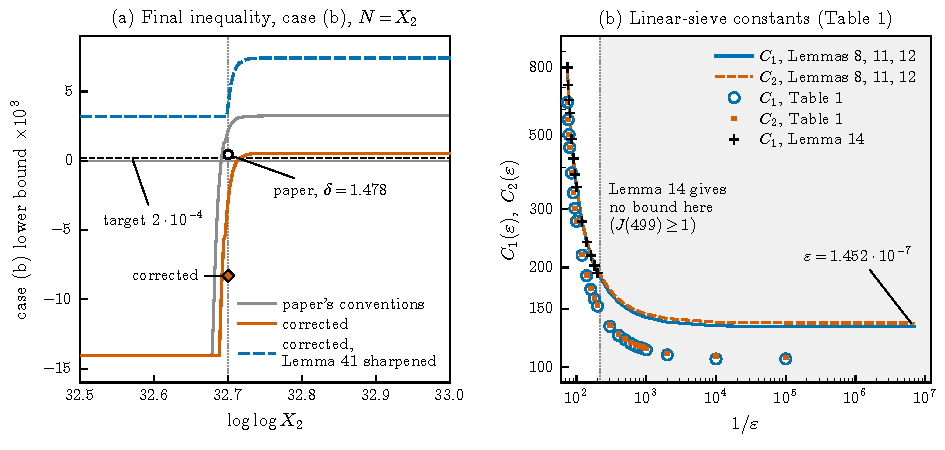
\includegraphics[width=0.82\textwidth]{figures/fig_bjs_chen_audit.pdf}
\caption{(a) Case-(b) lower bound for $\pi_2(N)/(U_NN/\log^2N)$ at $N=X_2$, with $X_3=X_2^{1/8}$ and the best
$\delta$ at each point (grid step $0.002$). Grey: the paper's conventions. Vermilion: with the three corrections
and the paper's lemmas. Blue: with Lemma~\ref{lem:sharp} as well. The dashed
line is the target $2\cdot10^{-4}$. (b) $C_1(\eps)$, $C_2(\eps)$ from Table~1 (markers) and from
Lemmas~8, 11 and~12 by direct summation (lines). Crosses: Lemma~14, which gives no bound in the shaded region
$1/\eps\ge219.4$.}
\label{fig:audit}
\end{figure}

\section{Scope}\label{sec:scope}

We read Section~2 and Sections~5--9 of \BJS{}. We transcribed the statements of Sections~4--8 that enter
the final inequality and recomputed every numerical constant in it. We did \emph{not} check the external explicit
inputs, which we used as quoted. These are Bordignon's bounds for exceptional zeros (the term
$100/(\sqrt K\log^2K)$ in $\nu$) and for primes in progressions ($3.2\cdot10^{-8}/\log^8x$, Lemma~27), Kadiri's
zero-free region ($R_0$, $R_1$), the Akbary--Hambrook estimate behind $27\,\mathcal E(y)$, and the bounds of
Broadbent et al., Büthe, Rosser--Schoenfeld, Montgomery--Vaughan and Johnston--Yang. We also did not check
Nathanson's Lemma~9.7 ($c_n\le0.9607$) and Theorems~9.3 and~10.2. We did not re-derive the proofs of Lemmas~29--36
and~38--43; we took their numerical constants as printed. The one new argument is Lemma~\ref{lem:sharp}.

\begin{thebibliography}{9}
\bibitem{BJS} M.~Bordignon, D.~R.~Johnston and V.~Starichkova, \emph{An explicit version of Chen's theorem and the
linear sieve}, Int.\ J.\ Number Theory \textbf{21} (2025), no.~10, 2497--2572,
\href{https://doi.org/10.1142/S1793042125501192}{doi:10.1142/S1793042125501192}; arXiv:2207.09452.
\bibitem{Chen} J.~R.~Chen, \emph{On the representation of a larger even integer as the sum of a prime and the
product of at most two primes}, Sci.\ Sinica \textbf{16} (1973), 157--176.
\bibitem{Nathanson} M.~B.~Nathanson, \emph{Additive Number Theory: The Classical Bases}, Graduate Texts in
Math.\ 164, Springer, 1996.
\end{thebibliography}

\end{document}
